\chapter{PENGUJIAN DAN ANALISIS}
\label{chap:pengujiananalisis}

% Ubah bagian-bagian berikut dengan isi dari pengujian dan analisis

Penelitian dilakukan dengan melakukan uji dan anaisa dari sistem yang telah dibuat berdasarkan langkah pada metodologi yang telah dilaksanakan. Pengujian ini dilakukan untuk menguji kemampuan sistem yang telah dibuat dalam menjawab permasalahan yang dijadikan acuan pada penelitian ini untuk mendapatkan hasil dari tujuan yang ingin didapat. Pembahasan pengujian yang dilakukan pada penelitian ini meliputi pengujian hasil \emph{training} dan \emph{validation} model, pengujian hasil \emph{testing} model, pengujian hasil deteksi dan pengujian prediksi.

\section{Pengujian Hasil \emph{Ttraining} dan \emph{Validation} Model}
\label{sec:PengujianTrainingValidation}

Pengujian pembuatan model berdasarkan hasil \emph{training} dan \emph{validation} dengan menggunakan dataset dengan jumlah keseluruhan yaitu 1731 sampel data. Dengan jumlah sample training sebanyak 1385 dan sampel validation sebanyak 346. Setelah dilakukan proses \emph{training} dan \emph{validation} terhadap dataset yang telah ditentukan oleh sampel data, didapatkan hasil pengujian akurasi dengan tingkat akurasi training sebesar 0,951 dan tingkat akurasi validation sebesar 0,977. Kemudian didapatkan hasil pengujian loss pada training sebesar 0,127 dan loss pada validation sebesar 0,059. Hasil pengujian ditunjukkan pada grafik nilai akurasi dan loss pada proses \emph{training} dan \emph{validation} seperti pada Gambar \ref{fig:HasilTrainingValidation}.

\begin{figure}[H]
  \centering
  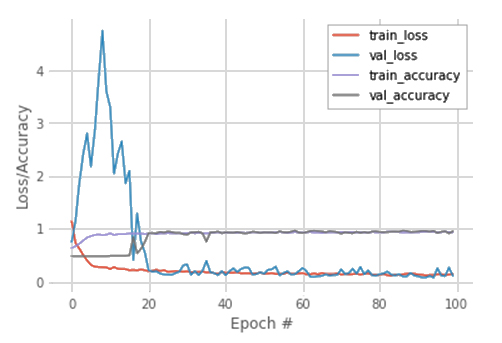
\includegraphics[scale=0.65]{gambar/hasil training dan validation w.jpg}
  \caption{Grafik hasil \emph{training} dan \emph{validation}}
  \label{fig:HasilTrainingValidation}
\end{figure}


\section{Pengujian Testing Model}
\label{sec:PengujianTestingModel}

Pengujian dilanjutkan dengan melakukan \emph{testing} model dengan menggunakan dataset yang sudah dimiliki dengan jumlah keseluruhan yaitu 347 sampel data. Dataset yang digunakan merupakan dataset yang sudah dilakukan filtrasi yang hanya digunakan pada pengujian \emph{testing} saja. Hasil pengujian \emph{testing} model didapatkan akurasi sebesar 95\% dengan hasil deteksi benar untuk kelas kanan sebanyak 170 sampel 96\% dan kelas kiri sebanyak 161 sampel 95\%. Pengujian ditunjukkan dengan confusion matrix pada Gambar \ref{fig:HasilTesting} dan Tabel \ref{tb:ClassificationReport} merupakan classification report dari hasil pengujian yang telah dilakukan pada pengujian \emph{testing} model penelitian ini.

\begin{figure}[H]
  \centering
  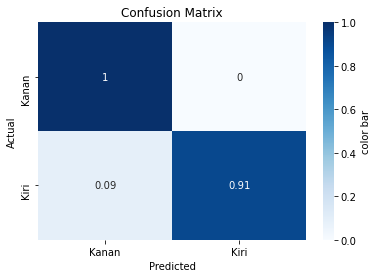
\includegraphics[scale=1]{gambar/cm normalized.png}
  \caption{\emph{Confusion Matrix} hasil \emph{testing} model}
  \label{fig:HasilTesting}
\end{figure}

\begin{longtable}{|c|c|c|c|c|}
  \caption{\emph{Classification Report} hasil pengujian \emph{testing} model}
  \label{tb:ClassificationReport}                                   \\
  \hline
  \rowcolor[HTML]{C0C0C0}
   & \textbf{Precision} & \textbf{Recall} & \textbf{F1-Score} & \textbf{Support} \\
  \hline
  kanan     & 0,91    & 1,00    & 0,96    & 170         \\
  \hline
  kiri      & 1,00    & 0,91    & 0,95    & 177           \\
  \hline
  Accuracy  &         &         & 0,95    & 347            \\
  \hline
\end{longtable}

\section{Pengujian Hasil Deteksi}
\label{sec:PengujianDeteksi}

Proses deteksi yang dilakukan dengan menggunakan model yang telah dibuat dilakukan pengujian dari hasil yang didapat dari hasil deteksi dengan perhitungan yang sebenarnya. Pengujian dilakukan dengan membuat data sebenarnya dengan melakukan perhitungan langkah dari akuisisi maupun data video yang digunakan dalam percobaan dan dibandingkan dengan hasil perhitungan langkah dari hasil deteksi. Tabel \ref{tb:PengujianDeteksi} menunjukkan hasil perhitungan data sebenarnya dengan data hasil deteksi terhadap langkah pada data video. 

\begin{longtable}{|c|c|c|}
  \caption{Pengujian Hasil Deteksi}
  \label{tb:PengujianDeteksi}                                   \\
  \hline
  \rowcolor[HTML]{C0C0C0}
  \textbf{Percobaan} & \textbf{Langkah} & \textbf{Deteksi Langkah} \\
  \hline
  1   & 241   & 328    \\
  \hline
  2   & 169   & 170    \\
  \hline
  3   & 302   & 302    \\
  \hline
  4   & 246   & 248    \\
  \hline
  5   & 321   & 322    \\
  \hline
  6   & 220   & 218    \\
  \hline
\end{longtable}

Pengujian dilakukan setelah didapatkan data hasil deteksi yang telah didapat dan juga data sebenarnya berdasarkan hasil perhitungan yang dilakukan terhadap data video. Setiap percobaan dilakukan analisa terkait perbandingan hasil yang didapat antara data hasil deteksi dan data perhitungan sebenarnya. Perbandingan dilakukan dengan mencari nilai error dari hasil perbedaan yang didapat dan dikalkulasikan dalam hasil akurasi dan error yang didapat dari analisa tersebut. Hasil analisa yang didapat dengan melakukan analisa pengujian hasil deteksi didapatkan hasil akurasi sebesar 99,36\% dengan hasil error sebesar 0,64\%. Tabel \ref{tb:AnalisaDeteksi} menunjukkan hasil analisa dari setiap percobaan yang dilakukan analisa pengujian.

\begin{longtable}{|c|c|c|c|c|c|}
  \caption{Analisa Pengujian Hasil Deteksi}
  \label{tb:AnalisaDeteksi}                                   \\
  \hline
  \rowcolor[HTML]{C0C0C0}
  \textbf{Percobaan} & \textbf{Langkah} & \textbf{Deteksi Langkah} & \textbf{Error} & \textbf{Error\%} & \textbf{Akurasi\%} \\
  \hline
  1   & 241   & 328 & 3   & 1,24\%    & 98,76\%   \\
  \hline
  2   & 169   & 170 & 1   & 0,59\%    & 99,41\%   \\
  \hline
  3   & 302   & 302 & 0   & 0\%       & 100\%     \\
  \hline
  4   & 246   & 248 & 2   & 0,81\%    & 99,19\%   \\
  \hline
  5   & 321   & 322 & 1   & 0,31\%    & 99,69\%   \\
  \hline
  6   & 220   & 218 & 2   & 0,91\%    & 99,09\%   \\
  \hline
\end{longtable}


\section{Pengujian Prediksi}
\label{sec:PengujianPrediksi}

Pengujian pada prediksi jumlah kalori yang terbakar dilakukan setelah melakukan pengujian pada model deteksi yang telah dilakukan. Prediksi dilakukan dengan dua metode, yaitu regresi linear dan perhitungan rumus. Dengan menggunakan dataset berupa citra video yang akan digunakan untuk melakukan prediksi kalori sebanyak 6 sampel video sehingga terdapat 6 percobaan yang dilakukan. Pada pengujian dengan regresi linear dengan melakukan proses deteksi dan menggunakan model regresi linear dalam melakukan proses prediksi kalori didapatkan beberapa data pendukung dalam hasil deteksi dan data dari hasil regresi prediksi kalori. Tabel \ref{tb:PengujianPrediksiRegresi} menunjukkan hasil deteksi dan hasil prediksi kalori dengan menggunakan regresi linear.

\begin{longtable}{|c|c|c|c|c|}
  \caption{Pengujian Prediksi dengan Regresi Linear}
  \label{tb:PengujianPrediksiRegresi}                                   \\
  \hline
  \rowcolor[HTML]{C0C0C0}
  \textbf{Percobaan} & \textbf{Deteksi Langkah} & \textbf{Jarak} & \textbf{Waktu} & \textbf{Kalori} \\
  \hline
  1   & 238   & 167,181    & 2:50    & 11,652  \\
  \hline
  2   & 170   & 118,437    & 1:35    & 8,245   \\
  \hline
  3   & 302   & 293,143    & 2:02    & 20,534  \\
  \hline
  4   & 248   & 284,417    & 1:41    & 19,927  \\
  \hline
  5   & 322   & 287,577    & 2:03    & 20,14   \\
  \hline
  6   & 218   & 286,18     & 1:21    & 20,056  \\
  \hline
\end{longtable}

Analisa pengujian \lipsum[1][1-3]. Tabel \ref{tb:AnalisaPrediksiRegresi} menunjukkan hasil analisa pengujian dari prediksi kalori dengan regresi linear.

\begin{longtable}{|c|c|c|c|c|c|}
  \caption{Analisa Pengujian Prediksi dengan Regresi Linear}
  \label{tb:AnalisaPrediksiRegresi}                                   \\
  \hline
  \rowcolor[HTML]{C0C0C0}
  \textbf{Percobaan} & \textbf{Kalori Treadmill} & \textbf{Prediksi Kalori} & \textbf{Error} & \textbf{Error\%} & \textbf{Akurasi\%} \\
  \hline
  1   & 10   & 11,652   & 1,652    & 16,52\%     & 83,48\%   \\
  \hline
  2   & 10   & 8,245    & 1,755    & 17,55\%     & 82,45\%   \\
  \hline
  3   & 20   & 20,534   & 0,534    & 2,67\%      & 97,33\%   \\
  \hline
  4   & 20   & 19,927   & 0,073    & 0,365\%     & 99,635\%  \\
  \hline
  5   & 20   & 20,14    & 0,14     & 0,7\%       & 99,3\%    \\
  \hline
  6   & 20   & 20,056   & 0,056    & 0,28\%      & 99,72\%   \\
  \hline
\end{longtable}

Pada pengujian dengan perhitungan rumus berdasarkan MET dilakukan dengan melalui proses deteksi dan melakukan perhitungan rumus menghasilkan beberapa data pendukung dalam perhitungan rumus dan hasil prediksi kalori yang didapat. Tabel \ref{tb:PengujianPrediksiPerhitungan} menunjukkan hasil deteksi dan hasil prediksi kalori dengan menggunakan perhitungan rumus.

\begin{longtable}{|c|c|c|c|c|}
  \caption{Pengujian Prediksi dengan Perhitungan Rumus}
  \label{tb:PengujianPrediksiPerhitungan}                                   \\
  \hline
  \rowcolor[HTML]{C0C0C0}
  \textbf{Percobaan} & \textbf{Deteksi Kecepatan} & \textbf{MET} & \textbf{Waktu} & \textbf{Kalori} \\
  \hline
  1   & 3,626   & 2,003    & 2:50    & 6,788   \\
  \hline
  2   & 5,016   & 2,733    & 1:35    & 4.744   \\
  \hline
  3   & 8,943   & 9,323    & 2:02    & 22.462  \\
  \hline
  4   & 10,893  & 10,721   & 1:41    & 20.575  \\
  \hline
  5   & 8,151   & 8,533    & 2:03    & 22.126  \\
  \hline
  6   & 13,041  & 11,985   & 1:21    & 19.331  \\
  \hline
\end{longtable}

Analisa pengujian \lipsum[1][1-4]. Tabel \ref{tb:AnalisaPrediksiPerhitungan} menunjukkan hasil analisa pengujian dari prediksi kalori dengan perhitungan rumus.

\begin{longtable}{|c|c|c|c|c|c|}
  \caption{Analisa Pengujian Prediksi dengan Perhitungan Rumus}
  \label{tb:AnalisaPrediksiPerhitungan}                                   \\
  \hline
  \rowcolor[HTML]{C0C0C0}
  \textbf{Percobaan} & \textbf{Kalori Treadmill} & \textbf{Prediksi Kalori} & \textbf{Error} & \textbf{Error\%} & \textbf{Akurasi\%} \\
  \hline
  1   & 10   & 6,788 & 3,212    & 32,12\%     & 67,88\%   \\
  \hline
  2   & 10   & 4,744 & 5,251    & 52,56\%     & 47,44\%   \\
  \hline
  3   & 20   & 22,462 & 2,462   & 12,31\%     & 87,69\%   \\
  \hline
  4   & 20   & 20,575 & 0,575   & 2,86\%      & 91,14\%   \\
  \hline
  5   & 20   & 22,126 & 2,126   & 10,63\%     & 89,37\%   \\
  \hline
  6   & 20   & 19,311 & 0,669   & 3,35\%      & 96,65\%   \\
  \hline
\end{longtable}

Hasil yang diperoleh melalui model yang telah dibuat untuk deteksi dan melakukan prediksi sesuai metode yang dilakukan didapatkan hasil akumulasi kalori dengan prediksi regresi sebesar 93,61\% dengan akumulasi error sebesar 6,39\%. Kemudian prediksi dengan perhitungan rumus didapatkan hasil akumulasi akurasi kalori sebesar 81,03\% dengan akumulasi error sebesar 18,97\%. Tabel \ref{tb:PengujianPrediksi} merupakan hasil perbandingan antara dataset percobaan dengan nilai kalori pembanding dataset dengan proses prediksi.

\begin{longtable}{|c|c|c|c|c|}
  \caption{Pengujian Hasil Prediksi Kalori}
  \label{tb:PengujianPrediksi}                                   \\
  \hline
  \rowcolor[HTML]{C0C0C0}
  \textbf{Percobaan} & \textbf{Kecepatan} & \textbf{Kalori Treadmill} & \textbf{Prediksi Regresi} & \textbf{Perhitungan MET} \\
  \hline
  1   & 3     & 10    & 11,652    & 6,788   \\
  \hline
  2   & 6     & 10    & 8,245     & 4,744   \\
  \hline
  3   & 9     & 20    & 20,534    & 22,462   \\
  \hline
  4   & 12    & 20    & 19,927    & 20,575   \\
  \hline
  5   & 8     & 20    & 20,14     & 22,126   \\
  \hline
  6   & 12    & 20    & 20,056    & 19,331   \\
  \hline
\end{longtable}